\subsection{Simultaneous\-Fit  Class Reference}
\label{class_simultaneousfit}\index{SimultaneousFit@{Simultaneous\-Fit}}
Simultaneous fitting of Vignets. 


{\tt \#include $<$simultaneousfit.h$>$}

Inheritance diagram for Simultaneous\-Fit::\begin{figure}[H]
\begin{center}
\leavevmode
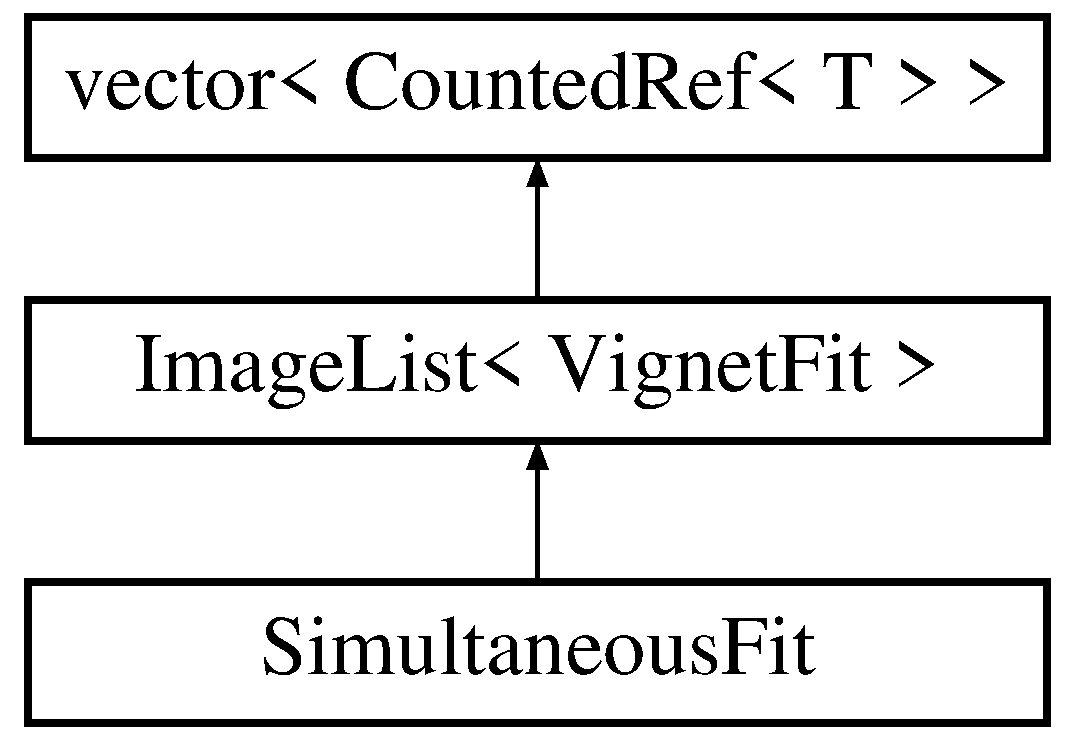
\includegraphics[height=3cm]{class_simultaneousfit}
\end{center}
\end{figure}
\subsubsection*{Public Methods}
\begin{CompactItemize}
\item 
\index{SimultaneousFit@{SimultaneousFit}!SimultaneousFit@{Simultaneous\-Fit}}\index{SimultaneousFit@{SimultaneousFit}!SimultaneousFit@{Simultaneous\-Fit}}
{\bf Simultaneous\-Fit} ()\label{class_simultaneousfit_a0}

\item 
\index{~SimultaneousFit@{$\sim$SimultaneousFit}!SimultaneousFit@{Simultaneous\-Fit}}\index{SimultaneousFit@{SimultaneousFit}!~SimultaneousFit@{$\sim$Simultaneous\-Fit}}
{\bf $\sim$Simultaneous\-Fit} ()\label{class_simultaneousfit_a1}

\item 
\index{FillMatAndVec@{FillMatAndVec}!SimultaneousFit@{Simultaneous\-Fit}}\index{SimultaneousFit@{SimultaneousFit}!FillMatAndVec@{Fill\-Mat\-And\-Vec}}
void {\bf Fill\-Mat\-And\-Vec} ()\label{class_simultaneousfit_a2}

\begin{CompactList}\small\item\em fill the entire matrix and vectors.\item\end{CompactList}\item 
\index{Solve@{Solve}!SimultaneousFit@{Simultaneous\-Fit}}\index{SimultaneousFit@{SimultaneousFit}!Solve@{Solve}}
bool {\bf Solve} (const double \&lambda=0, const bool invert=false)\label{class_simultaneousfit_a3}

\begin{CompactList}\small\item\em solve the linear equation system.\item\end{CompactList}\item 
\index{IterateAndSolve@{IterateAndSolve}!SimultaneousFit@{Simultaneous\-Fit}}\index{SimultaneousFit@{SimultaneousFit}!IterateAndSolve@{Iterate\-And\-Solve}}
bool {\bf Iterate\-And\-Solve} (const int Max\-Iterations, const double Epsilon=0.01)\label{class_simultaneousfit_a4}

\begin{CompactList}\small\item\em iterate on solution and solve the system.\item\end{CompactList}\item 
\index{AssignStar@{AssignStar}!SimultaneousFit@{Simultaneous\-Fit}}\index{SimultaneousFit@{SimultaneousFit}!AssignStar@{Assign\-Star}}
void {\bf Assign\-Star} ()\label{class_simultaneousfit_a5}

\begin{CompactList}\small\item\em assign the Vignet\-Fit star.\item\end{CompactList}\item 
\index{ComputeChi2@{ComputeChi2}!SimultaneousFit@{Simultaneous\-Fit}}\index{SimultaneousFit@{SimultaneousFit}!ComputeChi2@{Compute\-Chi2}}
double {\bf Compute\-Chi2} ()\label{class_simultaneousfit_a6}

\begin{CompactList}\small\item\em compute total chi2 and residuals of the fit.\item\end{CompactList}\item 
\index{ApplyCorrections@{ApplyCorrections}!SimultaneousFit@{Simultaneous\-Fit}}\index{SimultaneousFit@{SimultaneousFit}!ApplyCorrections@{Apply\-Corrections}}
bool {\bf Apply\-Corrections} (const double Factor=1)\label{class_simultaneousfit_a7}

\begin{CompactList}\small\item\em apply corrections of the last solution with a scale factor.\item\end{CompactList}\item 
\index{MakeResidsAndWeights@{MakeResidsAndWeights}!SimultaneousFit@{Simultaneous\-Fit}}\index{SimultaneousFit@{SimultaneousFit}!MakeResidsAndWeights@{Make\-Resids\-And\-Weights}}
void {\bf Make\-Resids\-And\-Weights} ()\label{class_simultaneousfit_a8}

\begin{CompactList}\small\item\em update all vignets from last model fitted and resid.\item\end{CompactList}\item 
\index{MakePsfs@{MakePsfs}!SimultaneousFit@{Simultaneous\-Fit}}\index{SimultaneousFit@{SimultaneousFit}!MakePsfs@{Make\-Psfs}}
void {\bf Make\-Psfs} ()\label{class_simultaneousfit_a9}

\begin{CompactList}\small\item\em redo all vignets integrated and convolved psfs and derivatives at the last fitted position.\item\end{CompactList}\item 
\index{DoTheFit@{DoTheFit}!SimultaneousFit@{Simultaneous\-Fit}}\index{SimultaneousFit@{SimultaneousFit}!DoTheFit@{Do\-The\-Fit}}
void {\bf Do\-The\-Fit} (const double \&Max\-Scale=1)\label{class_simultaneousfit_a10}

\begin{CompactList}\small\item\em fill, fit and shit.\item\end{CompactList}\item 
\index{SetWhatToFit@{SetWhatToFit}!SimultaneousFit@{Simultaneous\-Fit}}\index{SimultaneousFit@{SimultaneousFit}!SetWhatToFit@{Set\-What\-To\-Fit}}
void {\bf Set\-What\-To\-Fit} (const int To\-Fit=Fit\-Flux$|$Fit\-Gal)\label{class_simultaneousfit_a11}

\begin{CompactList}\small\item\em set what you want to fit.\item\end{CompactList}\item 
\index{FindMinimumScale@{FindMinimumScale}!SimultaneousFit@{Simultaneous\-Fit}}\index{SimultaneousFit@{SimultaneousFit}!FindMinimumScale@{Find\-Minimum\-Scale}}
void {\bf Find\-Minimum\-Scale} (const double \&Worst\-Seeing)\label{class_simultaneousfit_a12}

\begin{CompactList}\small\item\em get the minimum scaling factor to resize the vignets.\item\end{CompactList}\item 
\index{MakeInitialModel@{MakeInitialModel}!SimultaneousFit@{Simultaneous\-Fit}}\index{SimultaneousFit@{SimultaneousFit}!MakeInitialModel@{Make\-Initial\-Model}}
void {\bf Make\-Initial\-Model} ()\label{class_simultaneousfit_a13}

\begin{CompactList}\small\item\em build a rough initial galaxy to start the iterative fit.\item\end{CompactList}\item 
\index{Resize@{Resize}!SimultaneousFit@{Simultaneous\-Fit}}\index{SimultaneousFit@{SimultaneousFit}!Resize@{Resize}}
void {\bf Resize} (const double \&Scale\-Factor)\label{class_simultaneousfit_a14}

\begin{CompactList}\small\item\em resize all the vignets of a scale factor.\item\end{CompactList}\item 
\index{GetGalaxyFlux@{GetGalaxyFlux}!SimultaneousFit@{Simultaneous\-Fit}}\index{SimultaneousFit@{SimultaneousFit}!GetGalaxyFlux@{Get\-Galaxy\-Flux}}
double {\bf Get\-Galaxy\-Flux} (double \&Var\-Gal\-Flux) const\label{class_simultaneousfit_a15}

\begin{CompactList}\small\item\em compute galaxy flux consistently with the rest.\item\end{CompactList}\item 
\index{GetZeroFlux@{GetZeroFlux}!SimultaneousFit@{Simultaneous\-Fit}}\index{SimultaneousFit@{SimultaneousFit}!GetZeroFlux@{Get\-Zero\-Flux}}
double {\bf Get\-Zero\-Flux} (double \&Var\-Zero\-Flux) const\label{class_simultaneousfit_a16}

\begin{CompactList}\small\item\em compute zero flux as weighted average of zero nights.\item\end{CompactList}\item 
\index{write@{write}!SimultaneousFit@{Simultaneous\-Fit}}\index{SimultaneousFit@{SimultaneousFit}!write@{write}}
void {\bf write} (const string \&Middle\-Name) const\label{class_simultaneousfit_a17}

\begin{CompactList}\small\item\em write.\item\end{CompactList}\item 
\index{Chi2@{Chi2}!SimultaneousFit@{Simultaneous\-Fit}}\index{SimultaneousFit@{SimultaneousFit}!Chi2@{Chi2}}
double {\bf Chi2} () const\label{class_simultaneousfit_a18}

\begin{CompactList}\small\item\em returns total chi2 of the fit.\item\end{CompactList}\item 
\index{GetChi2@{GetChi2}!SimultaneousFit@{Simultaneous\-Fit}}\index{SimultaneousFit@{SimultaneousFit}!GetChi2@{Get\-Chi2}}
void {\bf Get\-Chi2} (double \&newchi2, const double \&oldchi2, double \&lambda)\label{class_simultaneousfit_a19}

\item 
\index{Dof@{Dof}!SimultaneousFit@{Simultaneous\-Fit}}\index{SimultaneousFit@{SimultaneousFit}!Dof@{Dof}}
int {\bf Dof} () const\label{class_simultaneousfit_a20}

\begin{CompactList}\small\item\em returns number of degrees of freedom.\item\end{CompactList}\item 
\index{Scale@{Scale}!SimultaneousFit@{Simultaneous\-Fit}}\index{SimultaneousFit@{SimultaneousFit}!Scale@{Scale}}
double {\bf Scale} () const\label{class_simultaneousfit_a21}

\begin{CompactList}\small\item\em returns the current scale factor for vignets.\item\end{CompactList}\end{CompactItemize}
\subsubsection*{Public Attributes}
\begin{CompactItemize}
\item 
\index{Minim@{Minim}!SimultaneousFit@{Simultaneous\-Fit}}\index{SimultaneousFit@{SimultaneousFit}!Minim@{Minim}}
Minim\-Method {\bf Minim}\label{class_simultaneousfit_m0}

\item 
\index{VignetRef@{VignetRef}!SimultaneousFit@{Simultaneous\-Fit}}\index{SimultaneousFit@{SimultaneousFit}!VignetRef@{Vignet\-Ref}}
Vignet\-Fit$\ast$ {\bf Vignet\-Ref}\label{class_simultaneousfit_m1}

\begin{CompactList}\small\item\em pointer to the best seeing vignet.\item\end{CompactList}\item 
\index{galaxy@{galaxy}!SimultaneousFit@{Simultaneous\-Fit}}\index{SimultaneousFit@{SimultaneousFit}!galaxy@{galaxy}}
{\bf Vignet}$\ast$ {\bf galaxy}\label{class_simultaneousfit_m2}

\begin{CompactList}\small\item\em pointer to the reconstructed galaxy centered double image.\item\end{CompactList}\end{CompactItemize}


\subsubsection{Detailed Description}
Simultaneous fitting of Vignets.



The documentation for this class was generated from the following file:\begin{CompactItemize}
\item 
{\bf simultaneousfit.h}\end{CompactItemize}
